\documentclass[french, a4paper, 12pt, twocolumn, landscape]{article}



%% Langue et compilation

\usepackage[utf8]{inputenc}
\usepackage[T1]{fontenc}
\usepackage[french]{babel}

%% LISTE DES PACKAGES

\usepackage{mathtools}     % package de base pour les maths
\usepackage{amsmath}       % mathematical type-setting
\usepackage{amssymb}       % symbols speciaux pour les maths
\usepackage{textcomp}      % symboles speciaux pour el text
\usepackage{gensymb}       % commandes generiques \degree etc...
\usepackage{tikz}          % package graphique
\usepackage{wrapfig}       % pour entourer a cote d'une figure
\usepackage{color}         % package des couleurs
\usepackage{xcolor}        % autre package pour les couleurs
\usepackage{pgfplots}      % pacakge pour creer des graph
\usepackage{epsfig}        % permet d'inclure des graph en .eps
\usepackage{graphicx}      % arguments dans includegraphics
\usepackage{pdfpages}      % permet d'insérer des pages pdf dans le document
\usepackage{subfig}        % permet de creer des sous-figure
\usepackage{pst-all}       % utile pour certaines figures en pstricks
\usepackage{lipsum}        % package qui permet de faire des essais
\usepackage{array}         % permet de faire des tableaux
\usepackage{multicol}      % plusieurs colonnes sur une page
\usepackage{enumitem}      % pro­vides user con­trol: enumerate, itemize and description
\usepackage{hyperref}      % permet de creer des hyperliens dans le document
\usepackage{lscape}        % permet de mettre une page en mode paysage
\usepackage{lmodern}       % permet d'avoir certains "fonts" de bonen qualite
\usepackage{fancyhdr}      % Permet de mettre des informations en hau et en bas de page      
\usepackage[framemethod=tikz]{mdframed} % breakable frames and coloured boxes
\usepackage[top=1.5cm, bottom=1.5cm, left=2.5cm, right=2.5cm]{geometry} % donne les marges
\usepackage[font=normalsize, labelfont=bf,labelsep=endash, figurename=Fig.]{caption} % permet de changer les legendes des figures
\usepackage{lewis}
\usepackage{bohr}
\usepackage{chemfig}
\usepackage{chemist}

%% LIBRAIRIES

\usetikzlibrary{plotmarks} % librairie pour les graphes
\usetikzlibrary{patterns}  % necessaire pour certaines choses predefinies sur tikz
\usetikzlibrary{shadows}   % ombres des encadres
\usetikzlibrary{backgrounds} % arriere plan des encadres


%% MISE EN PAGE

\pagestyle{fancy}     % Défini le style de la page

\renewcommand{\headrulewidth}{1pt}      % largeur du trait en haut de la page
\fancyhead[L]{Seconde générale}         % info coin haut gauche
\fancyhead[R]{Lycée Jean Guéhenno}  % info coin haut droit

% bas de la page
\renewcommand{\footrulewidth}{1pt}      % largeur du trait en bas de la page
\fancyfoot[L]{G. \bsc{LE DOUDIC}}  % info coin bas gauche
\fancyfoot[R]{TP 4 : Famille chimique}                         % info coin bas droit


\setlength{\columnseprule}{1pt} 
\setlength{\columnsep}{30pt}



%% NOUVELLES COMMANDES 

\DeclareMathOperator{\e}{e} % permet d'ecrire l'exponentielle usuellement


\newcommand{\gap}{\vspace{0.15cm}}   % defini une commande pour sauter des lignes
\renewcommand{\vec}{\overrightarrow} % permet d'avoir une fleche qui recouvre tout le vecteur
\newcommand{\bi}{\begin{itemize}}    % begin itemize
\newcommand{\ei}{\end{itemize}}      % end itemize
\newcommand{\bc}{\begin{center}}     % begin center
\newcommand{\ec}{\end{center}}       % end center
\newcommand\opacity{1}               % opacity 
\pgfsetfillopacity{\opacity}

\newcommand*\Laplace{\mathop{}\!\mathbin\bigtriangleup} % symbole de Laplace

\frenchbsetup{StandardItemLabels=true} % je ne sais plus

\newcommand{\smallO}[1]{\ensuremath{\mathop{}\mathopen{}o\mathopen{}\left(#1\right)}} % petit o

\newcommand{\cit}{\color{blue}\cite} % permet d'avoir les citations de couleur bleues
\newcommand{\bib}{\color{black}\bibitem} % paragraphe biblio en noir et blanc
\newcommand{\bthebiblio}{\color{black} \begin{thebibliography}} % idem necessaire sinon bug a cause de la couleur
\newcommand{\ethebiblio}{\color{black} \end{thebibliography}}   % idem
%%% TIKZ


%% COULEURS 


\definecolor{definitionf}{RGB}{220,252,220}
\definecolor{definitionl}{RGB}{39,123,69}
\definecolor{definitiono}{RGB}{72,148,101}

\definecolor{propositionf}{RGB}{255,216,218}
\definecolor{propositionl}{RGB}{38,38,38}
\definecolor{propositiono}{RGB}{109,109,109}

\definecolor{theof}{RGB}{255,216,218}
\definecolor{theol}{RGB}{160,0,4}
\definecolor{theoo}{RGB}{221,65,100}

\definecolor{avertl}{RGB}{163,92,0}
\definecolor{averto}{RGB}{255,144,0}

\definecolor{histf}{RGB}{241,238,193}

\definecolor{metf}{RGB}{220,230,240}
\definecolor{metl}{RGB}{56,110,165}
\definecolor{meto}{RGB}{109,109,109}


\definecolor{remf}{RGB}{230,240,250}
\definecolor{remo}{RGB}{150,150,150}

\definecolor{exef}{RGB}{240,240,240}

\definecolor{protf}{RGB}{247,228,255}
\definecolor{protl}{RGB}{105,0,203}
\definecolor{proto}{RGB}{174,88,255}

\definecolor{grid}{RGB}{180,180,180}

\definecolor{titref}{RGB}{230,230,230}

\definecolor{vert}{RGB}{23,200,23}

\definecolor{violet}{RGB}{180,0,200}

\definecolor{copper}{RGB}{217, 144, 88}

%% Couleur des ref

\hypersetup{
	colorlinks=true,
	linkcolor=black,
	citecolor=blue,
	urlcolor=black
		   }

%% CADRES


% %%%%%%%%%% DEFINITION
% \newmdenv[tikzsetting={fill=definitionf}, linewidth=2pt, linecolor=definitionl, outerlinewidth=0pt, innertopmargin=5pt, innerbottommargin=5pt, innerleftmargin=5pt, innerrightmargin=5pt, leftmargin=0pt]{definition}

% \newmdenv[ tikzsetting={drop shadow={ shadow xshift=1ex, shadow yshift=-0.5em, fill=definitiono, opacity=1, every shadow } }, outerlinewidth=2pt, outerlinecolor=white, linecolor=white, innertopmargin=0pt, innerbottommargin=0pt, innerleftmargin=0pt, innerrightmargin=0pt]{ombredef}


% %%%%%%%%%% THEOREME

% \newmdenv[tikzsetting={fill=theof}, linewidth=2pt, linecolor=theol, outerlinewidth=0pt, innertopmargin=5pt, innerbottommargin=5pt, innerleftmargin=5pt, innerrightmargin=5pt, leftmargin=0pt]{theo}

% \newmdenv[ tikzsetting={drop shadow={ shadow xshift=1ex, shadow yshift=-0.5em, fill=theoo, opacity=1, every shadow } }, outerlinewidth=2pt, outerlinecolor=white, linecolor=white, innertopmargin=0pt, innerbottommargin=0pt, innerleftmargin=0pt, innerrightmargin=0pt]{ombretheo}


% %%%%%%%%%% METHODE

% \newmdenv[tikzsetting={fill=metf}, linewidth=2pt, linecolor=metl, outerlinewidth=0pt, innertopmargin=5pt, innerbottommargin=5pt, innerleftmargin=5pt, innerrightmargin=5pt, leftmargin=0pt]{met}

% \newmdenv[ tikzsetting={drop shadow={ shadow xshift=1ex, shadow yshift=-0.5em, fill=meto, opacity=1, every shadow } }, outerlinewidth=2pt, outerlinecolor=white, linecolor=white, innertopmargin=0pt, innerbottommargin=0pt, innerleftmargin=0pt, innerrightmargin=0pt]{ombremet}



%%%%%%%%%%% RQ

\newmdenv[tikzsetting={fill=remf}, linewidth=2pt, linecolor=remf, outerlinewidth=0pt, innertopmargin=5pt, innerbottommargin=5pt, innerleftmargin=5pt, innerrightmargin=5pt, leftmargin=0pt]{remarque}

\newmdenv[ tikzsetting={drop shadow={ shadow xshift=1ex, shadow yshift=-0.5em, fill=remo, opacity=1, every shadow } }, outerlinewidth=2pt, outerlinecolor=white, linecolor=white, innertopmargin=0pt, innerbottommargin=0pt, innerleftmargin=0pt, innerrightmargin=0pt]{ombreremarque}

%%%%%%%%%%% Cadre pour le titre

\tikzset{every shadow/.style={opacity=1}}

\global\mdfdefinestyle{doc}{backgroundcolor=white, shadow=true, shadowcolor=propositiono, linewidth=1pt, linecolor=black, shadowsize=5pt}
\global\mdfdefinestyle{titr}{backgroundcolor=metf, shadow=true, shadowcolor=propositiono, linewidth=1pt, linecolor=black, shadowsize=5pt}
\global\mdfdefinestyle{theo}{backgroundcolor=theof, shadow=true, shadowcolor=theoo, linewidth=1pt, linecolor=theol, shadowsize=5pt}
\global\mdfdefinestyle{prop}{backgroundcolor=theof, shadow=true, shadowcolor=propositiono, linewidth=1pt, linecolor=theol, shadowsize=5pt}
\global\mdfdefinestyle{def}{backgroundcolor=definitionf, shadow=true, shadowcolor=definitiono, linewidth=1pt, linecolor=definitionl, shadowsize=5pt}
\global\mdfdefinestyle{histo}{backgroundcolor=histf, shadow=true, shadowcolor=propositiono, linewidth=1pt, linecolor=black, shadowsize=5pt}
\global\mdfdefinestyle{avert}{backgroundcolor=white, shadow=true, shadowcolor=averto, linewidth=1pt, linecolor=avertl, shadowsize=5pt}
\global\mdfdefinestyle{met}{backgroundcolor=metf, shadow=true, shadowcolor=meto, linewidth=1pt, linecolor=metl, shadowsize=5pt}
\global\mdfdefinestyle{rem}{backgroundcolor=metf, shadow=true, shadowcolor=meto, linewidth=1pt, linecolor=metf, shadowsize=5pt}
\global\mdfdefinestyle{exo}{backgroundcolor=exef, shadow=true, shadowcolor=propositiono, linewidth=1pt, linecolor=exef, shadowsize=5pt}
\global\mdfdefinestyle{not}{backgroundcolor=definitionf, shadow=true, shadowcolor=propositiono, linewidth=1pt, linecolor=black, shadowsize=5pt}
\global\mdfdefinestyle{proto}{backgroundcolor=protf, shadow=true, shadowcolor=proto, linewidth=1pt, linecolor=protl, shadowsize=5pt}

%%%%%%
\definecolor{cobalt}{rgb}{0.0, 0.28, 0.67}
\definecolor{applegreen}{rgb}{0.55, 0.71, 0.0}

\usepackage{tcolorbox}
  \tcbuselibrary{most}
  \tcbset{colback=cobalt!5!white,colframe=cobalt!75!black}



\newtcolorbox{definition}[1]{
	colback=applegreen!5!white,
  	colframe=applegreen!65!black,
	fonttitle=\bfseries,
  	title={#1}}
\newtcolorbox{Programme}[1]{
	colback=cobalt!5!white,
  	colframe=cobalt!65!black,
	fonttitle=\bfseries,
  	title={#1}}  

\newtcolorbox{Exercice}[1]{
  colback=cobalt!5!white,
  colframe=cobalt!65!black,
  fonttitle=\bfseries,
  title={#1}}  

  \newtcolorbox{Protocol}[1]{
  colback=cyan!5!white,
  colframe=cyan!65!black,
  fonttitle=\bfseries,
  title={#1}}  

\newtcolorbox{Resultat}[1]{
	colback=theof,%!5!white,
	colframe=theoo!85!black,
  fonttitle=\bfseries,
	title={#1}} 	


\def\width{12}
\def\hauteur{5}

\setlength{\parskip}{0pt}%
\setlength{\parindent}{18pt}


%% MODIFICATION DE CHAPTER  
\makeatletter
\def\@makechapterhead#1{%
  %%%%\vspace*{50\p@}% %%% removed!
  {\parindent \z@ \raggedright \normalfont
    \ifnum \c@secnumdepth >\m@ne
        \huge\bfseries \@chapapp\space \thechapter
        \par\nobreak
        \vskip 20\p@
    \fi
    \interlinepenalty\@M
    \Huge \bfseries #1\par\nobreak
    \vskip 40\p@
  }}
\def\@makeschapterhead#1{%
  %%%%%\vspace*{50\p@}% %%% removed!
  {\parindent \z@ \raggedright
    \normalfont
    \interlinepenalty\@M
    \Huge \bfseries  #1\par\nobreak
    \vskip 40\p@
  }}
  
  \newcommand{\isotope}[3]{%
     \settowidth\@tempdimb{\ensuremath{\scriptstyle#1}}%
     \settowidth\@tempdimc{\ensuremath{\scriptstyle#2}}%
     \ifnum\@tempdimb>\@tempdimc%
         \setlength{\@tempdima}{\@tempdimb}%
     \else%
         \setlength{\@tempdima}{\@tempdimc}%
     \fi%
    \begingroup%
    \ensuremath{^{\makebox[\@tempdima][r]{\ensuremath{\scriptstyle#1}}}_{\makebox[\@tempdima][r]{\ensuremath{\scriptstyle#2}}}\text{#3}}%
    \endgroup%
  }%

\makeatother

\usepackage{eurosym}
\usepackage{colortbl}
% \onehalfspacing
%%
%% DEBUT DU DOCUMENT
%%
\begin{document}


%%%%%%

\titre{Chapitre 12 : Les transformations chimiques}

\doc{1}{Bulletin officiel}{
\begin{center}
	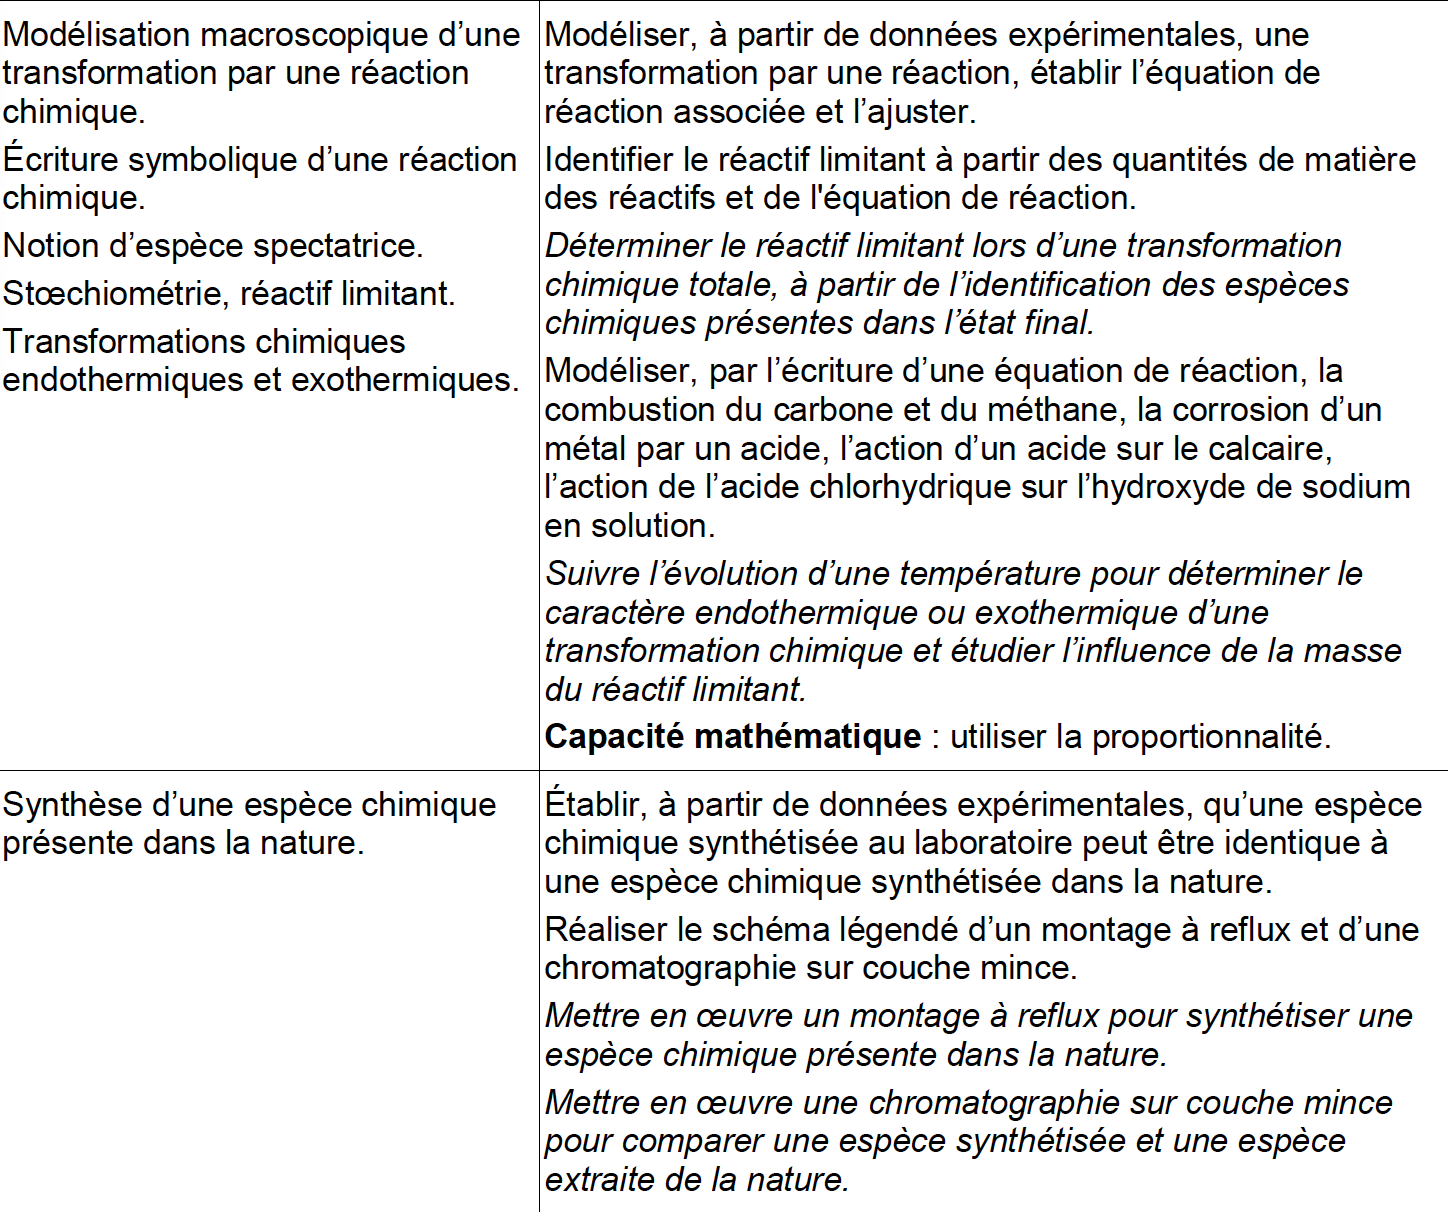
\includegraphics[width=.85\linewidth]{BO.png}
	
\end{center}
}


\doc{2}{Exercices dans le livre scolaire}{
		\begin{enumerate}
			\item Compétences de base : exercices 5,6, 11 page 154;
			\item Pour confirmer  : exercices 12, 13, 18 et 26 pages 154-157;
			\item Parcours expert : exercices 19 et 20 pages 157.
		\end{enumerate}
}\vspace{1cm}
	\noindent \textbf{Quiz sur les forces et principe d'inertie}
\begin{center}
	\begin{minipage}{.5\linewidth}
		\centering
		
\includegraphics[width=.2\linewidth]{Quiz1.png}
		
		Quiz 1 - Les transformations chimiques : \url{https://forms.office.com/r/US46AMq3KD?origin=lprLink}
	\end{minipage}\hfill
	\begin{minipage}{.5\linewidth}
		\centering
		
\includegraphics[width=.2\linewidth]{Quiz2.png}

		Quiz 2 - Ajuster des équations bilan: \url{https://forms.office.com/r/xJQKwRDU8z?origin=lprLink}
	\end{minipage}\\
\begin{minipage}{.5\linewidth}
			\centering
			
\includegraphics[width=.2\linewidth]{Quiz3.png}
	
			Quiz 3 - Le réactif limitant: \url{https://forms.office.com/r/HPNvx7VjLK?origin=lprLink}
		\end{minipage}\hfill
		\begin{minipage}{.5\linewidth}
			\centering
			
\includegraphics[width=.2\linewidth]{Quiz4.png}
	
			Quiz 4 - Les réactions exothermiques \url{https://forms.office.com/r/3VEZLAuQzk?origin=lprLink}
		\end{minipage}
 \end{center}

\section*{Introduction}

Durant une transformation chimiques, les atomes constituants les espèces chimiques s'associent différemment pour former de nouvelles espèces. Comment peut-on modéliser ces transformations  ? Lavoisier s'y est essayé au XVIIIe siècle, inspirant ainsi les chimistes jusqu'à aujourd'hui.

	\histo{Antoine Laurent de Lavoisier (1743-1794)}{

	\begin{minipage}{.6\linewidth}
		Il a énoncé le principe suivant : \og{} On peut poser en principe, que dans toute opération, il y a une égale quantité de matière avant et après l'opération, que la qualité et la quantité des principes est la même\fg{}.\medskip
	
	Il s'essaye à schématiser ces transformations en utilisant des symboles chimiques, des coefficients, des additions d'espèces.
	\end{minipage}\hfill
	\begin{minipage}{.3\linewidth}
\centering
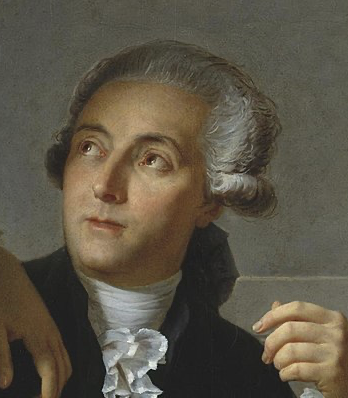
\includegraphics[width=.5\linewidth]{Lavoisier.png}
\captionof{figure}{Antoine Laurent de Lavoisier, \textit{cf wikipedia}}
\end{minipage}
}

\section{Modélisation des transformations chimiques}
\subsection{Le système chimique}

\begin{definition}{Définition 1 - Le système chimique}
	Un système chimique est formé d'espèces chimiques. Il est décrit par les caractéristiques suivantes:
	\begin{itemize}
		\item la nature des espèces chimiques;
		\item leur état physique : \textbf{solide} (s), \textbf{liquide} (l), \textbf{gaz} (g) ou \textbf{aqueux} (aq);
		\item leur quantité de matière ($n$);
		\item la température ($T$) et la pression ($P$)
	\end{itemize}
\end{definition}

\subsection{Observations macroscopiques}

\begin{minipage}{.63\linewidth}
	Au cours d'une \textbf{transformation chimique} des espèces chimiques se transforment en de nouvelles espèces. Les atomes de départs ne disparaissent pas seul leur organisation change. En observant une expérience, il est possible d'identifier les espèces chimiques qui se sont transformées.
\end{minipage}\hfill
\begin{minipage}{.32\linewidth}

	Disparition d'un réactif !

	\centering
	
\includegraphics[width=.5\linewidth]{AcideOxalique.png}
	\captionof{figure}{\url{https://dgxy.link/FkI0F}}
\end{minipage}

\begin{definition}{Définition 2 - Les réactifs et les produits}
	Les espèces chimiques qui se sont transformées sont appelées \textbf{réactifs} et \textbf{produits}. Les réactifs sont les espèces de départ. Les produits sont issus de la réorganisation des réactifs, ce sont les produits de la transformation chimique.
\end{definition}

\subsection{Écriture symbolique d'une réaction chimique}

Après avoir observé et listé les espèces chimiques présentes au cours d'une transformation chimique, il est possible d'indiquer quels sont les réactifs et les produits de la transformation en comparant l'état initial et final de la transformation. 

\begin{definition}{Définition 3 - L'équation bilan de la réaction}

	L'équation chimique \textbf{modélise} la transformation chimique microscopique ayant lieu. Elle indique donc les \textbf{réactifs} qui se transforment en \textbf{produits} à l'aide d'une flèche : 
	
	$$\rm réactif~1+réactif~2+\dots	 \rightarrow produits~1+produits~2+\dots$$
	
\end{definition}

\subsection{Notion d'espèce spectatrice}

\begin{definition}{Définition 3 - Espèce chimique spectatrice}

	Une espèce chimique qui est présente au cours de la réaction mais qui nesubit aucun changement est une espèce spectatrice.
	
\end{definition}

\textbf{Remarque:} Cette espèce ne subissant pas de transformation, elle n'apparaît pas dans l'équation bilan.
\exo{1}{Précipité bleu d'hydroxyde de cuivre}{On mélange de l'hydroxyde de sodium ($\rm Na^{+};HO^{-}$) et du sulfate de cuivre ($\rm Cu^{2+};SO_4^{2-}$) pour former du $\rm Cu(OH)_2$. Indiquer quelles sont les espèces spectatrices, les réactifs et les produits. Écrie l'équation bilan de la réaction :$\rm Cu^{2+} + 2HO^{-}\rightarrow Cu(OH)_2$, $\rm SO_4^{2-}$ et $\rm Na^{+}$ sont spectateurs.
}

\section{St\oe chiométrie de la réaction}


\subsection{Ajuster une équation de réaction}
D'après \bsc{Lavoisier}, le nombre et la nature des éléments sont conservés au cours d'une transformation, ainsi on doit retrouver avant et après la transformation les mêmes éléments chimiques et leur nombre.



\methode{1}{Ajuster une équation de réaction}{\textbf{Ajuster une équation chimique consiste à prendre en compte la st\oe chimoétrie de la réaction} et donc à indiquer les proportions des réactifs réagissant ensemble et celles des produits formés.}

\begin{center}
	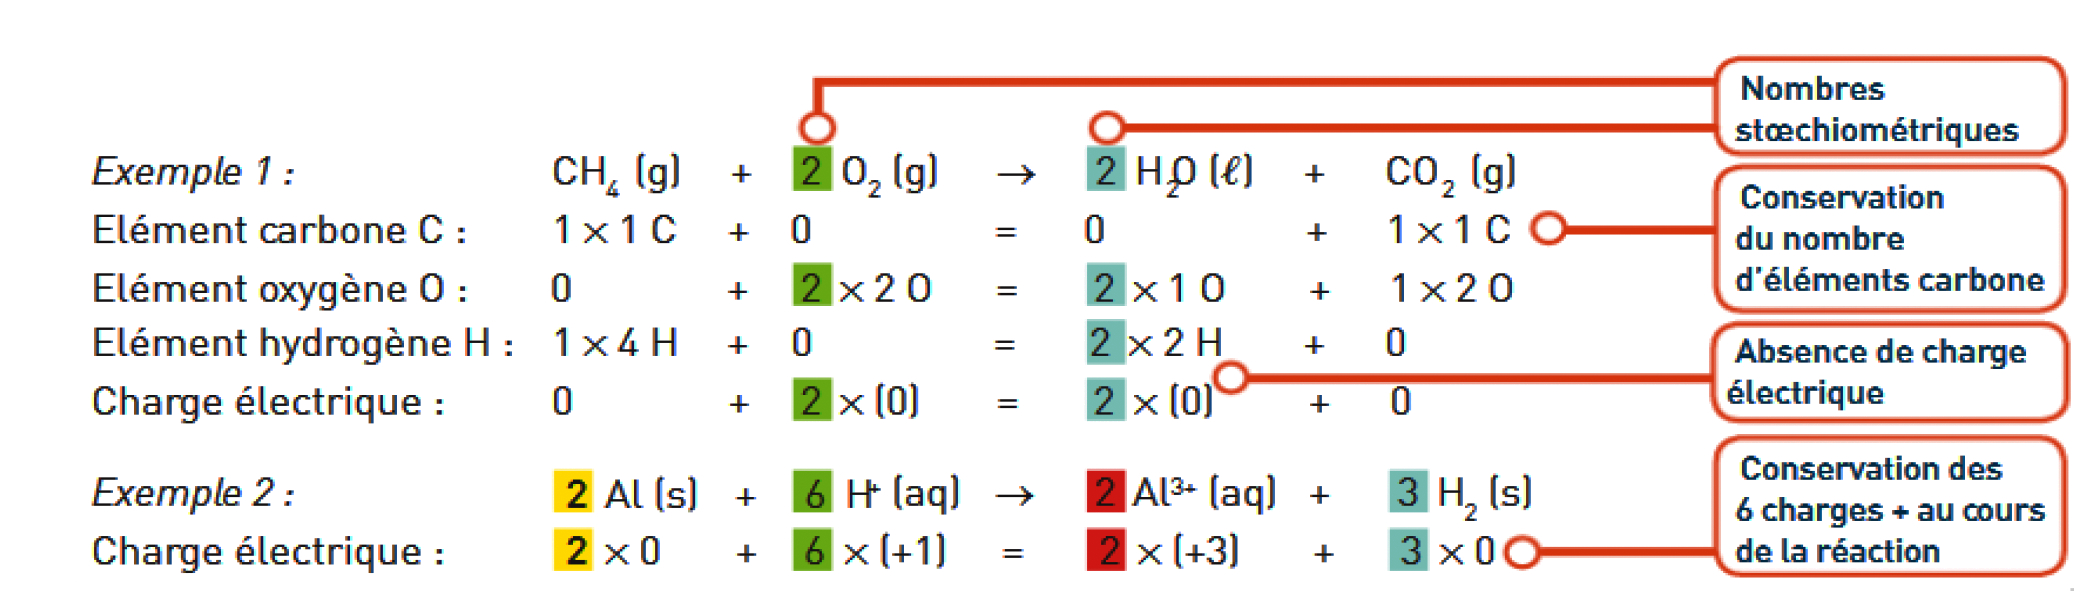
\includegraphics[width=\linewidth]{exempleAjustement.jpg}
\end{center}

\avert{}{Ne pas confondre !}{
	Le nombre st\oe chimoétrique, placé devant la formule est différent des indices placés dans la formule chimique. $\rm 2H_2O$ signifie $2\times H_2O$ : 4 atomes d'hydrogène et 2 atomes d'oxygène.
}


\exo{2}{Ajuster des équations chimiques sous forme de jeu}{\textbf{Consigne :} Rendez vous sur le site suivant : \url{https://dgxy.link/KCTmS} faites la partie introductive puis les jeux. Compléter au fur et à mesure les équations de réaction ci-dessous :

\begin{enumerate}
	\item Synthèse de l'ammoniac : 
	

	$$\large \rm 1 ~N_2 +~ 3~ H_2 \rightarrow ~ 2 ~NH_3$$

	\item Dissociation de l'eau : 
	
	$$\large \rm 2 ~H_2O \rightarrow ~2x~H_2 + ~1  ~O_2$$

	\item Combustion du méthane : 
	
	$$\large \rm 1~ CH_4+~2~O_2 \rightarrow ~1~CO_2+ ~2~H_2O$$

	\item Dissociation du gaz carbonique : 
	
	$$\large \rm 2  ~CO_2 \rightarrow 2 ~CO + 1~ O_2$$

	\item Sulfure de carbone en présence de dioxygène : 
	
	$$\large \rm 1 ~CS_2+~3 ~O_2 \rightarrow ~1 ~CO_2+ ~2 ~SO_2$$


	\item Combustion du butane
	
	$$\large \rm 2 ~C_2H_6+~7~O_2 \rightarrow ~4~CO_2+ ~2 ~6H_2O$$

	\item Combustion de l'éthanol
	
	$$\large \rm 1 ~C_2H_5OH+~3~O_2 \rightarrow ~2~CO_2+ ~2 ~3H_2O$$
	% \item Synthèse de l'ammoniac : 
	
	\item Synthèse de l'ammoniac 2 
	
	$$\large \rm 2 ~N_2+~6H_2O \rightarrow ~4~NH_3+ 3~0_2$$

	% \item Synthèse de l'ammoniac :
	% $$\large \rm \dots ~N_2 +~ \dots~ H_2 \rightarrow ~\dots ~NH_3$$

	% \item Dissociation de l'eau : 
	
	% $$\large \rm \dots ~H_2O \rightarrow ~\dots ~H_2 + ~\dots ~O_2$$

	% \item Combustion du méthane : 
	
	% $$\large \rm \dots ~CH_4+~\dots ~O_2 \rightarrow ~\dots~CO_2+ ~\dots ~H_2O$$

	% \item Dissociation du gaz carbonique : 
	
	% $$\large \rm \dots ~CO_2 \rightarrow ~\dots ~CO +~\dots ~O_2$$
\end{enumerate}
}

\subsection{Le réactif limitant}
Les nombres stoechiométriques nous renseignent sur les proportions de chacun des réactifs. Lorsque la réaction s’arrête, c’est qu’il n’y a plus de réactif pour réaliser la transformation. Seul un des ces réactifs peut-être responsable de cet arrêt.

\begin{definition}{Définition 4 - Le réactif limitant}
	\textbf{Le réactif limitant} est celui qui est \textbf{totalement} tansformé au cours de la réaction. Il est responsable de l'arrêt de la réaction.\footnote{Pour voir la notion de réactif limitant en vidéo aller voir le quiz numéro 3.}
\end{definition}

\textbf{Remarque :} Si les deux réactif sont présents en proportions stoechiométriques, c’est qu’il n’en reste aucun à la fin de la transformation. Il n’y a donc aucun réactif limitant.

\methode{2}{Comment déterminer le réactif limitant ?}{
Il faut comparer les quantités de matière de chacun des réactifs. Cela permet ensuite de calculer les quantités de produits formés et celles des réactifs restants.
}

\exo{3}{Réactif limitant dans la combustoin de propane}{On place dans la même enceinte $m_{propane}=50~\rm g$ de propane ($C_3H_{5(g)}$) en présence de $m_{dioxygène}=240~\rm g$ de dioxygène ($0_{2(g)}$). Une flamme permet de démarrer la combustion qui est modélisée par l'équation suivante : 

$$C_3H_{5(g)}+5O_{2(g)}\rightarrow 3CO_{2(g)}+4H_2O_{(g)}.$$ Déterminer quel est le réactif limitant sachant que 1 mole de propane correspond à 44 g, et 1 mole de dioxygène correspond à 32 g.\medskip

\textbf{Solution :}\medskip

\begin{itemize}
	\item Si une mole de propane correspond à 44g, alors les 50g de propane introduits dans l'enceinte correspondent à $n_{prop} = \dfrac{50(g)\times 1(mol)}{44 (g)} = 1,1~\rm mol$ de propane. 
	\item Si une mole de dioxygène correspond à 32g, alors les 240g de propane introduits dans l'enceinte correspondent à $\rm n_{dioxygène} = \dfrac{240(g)\times 1(mol)}{44 (g)} = 7,5~\rm mol$ de propane. 
\end{itemize}

Pour 1 mole de propane, on consomme 5 moles de dioxygène, ainsi $1,1$ mol de propane réagissent avec $5\times 1,1 = 5.5$ mol de dioxygène. Ce qui est inférieur à la quantité initiale de dioxygène.\medskip

Par conséquent ce n'est pas le dioxygène qui limitera la réaction mais le propane. 
}

\section{Effets thermiques d'une transformation chimique}


\begin{definition}{Définition 5 - Transformation endothermique et exothermique}
	Une transformation chimique qui nécessite une absorption d'énergie est \textbf{endothermique} : la température globale du système va diminuer.\medskip

	Une transformation chimique qui libère de l'énergie est \textbf{exothermique} : la température globale du système va augmenter.
\end{definition}

\begin{proposition}{Propriété 1 - Masse du réactif limitant}
	Plus la masse du réactif limitant est élevée, plus la variation de température observée sera significative.
\end{proposition}


\section{Synthèses d'espèces chimiques : pourquoi copier la nature ?}



\subsection{Espèces chimiques naturelles, synthétiques, artificielles}
\begin{definition}{Définition 6 - Synthétiser une espèce chimique}
	Synthétiser une espèce chimique signifie fabriquer une espèce chimique grâce à une transformation chimique.
\end{definition}

Nous pouvons distinguer trois catégories de molécules
\begin{itemize}
	\item Les molécules naturelles (extraites de la nature);
	\item Les molécules de synthèse  : identiques aux naturelles mais fabriquées par l'homme et copiées sur celles issues de la nature;
	\item Les molécules artificielles : fabriquées par l'homme, n'existant pas dans la nature.
\end{itemize}

\exo{4}{Attribué les images aux différents types de molécules}{

	
	\begin{minipage}{.3\linewidth}
		\centering

		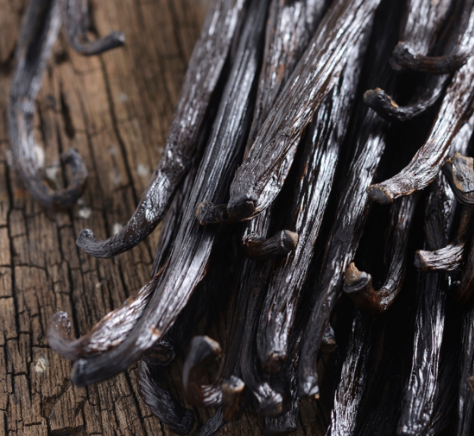
\includegraphics[width=.45\linewidth]{VanilleBourbon.png}
	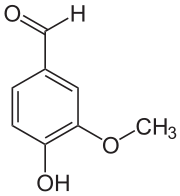
\includegraphics[width=.45\linewidth]{Vanillin_wiki.png}
	\captionof{figure}{La vanilline extraite des plantation sur l'île de la Réunion
	}
	\end{minipage}\hfill
	\begin{minipage}{.3\linewidth}
			\centering
	
\includegraphics[width=.4\linewidth]{CachetVitamineC.png}
	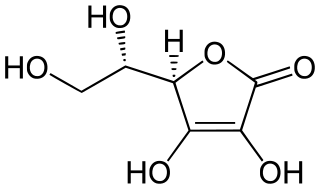
\includegraphics[width=.55\linewidth]{Ascorbique_wiki.png}
	\captionof{figure}{La vitamine C, présente dans les oranges}
	
	\end{minipage}\hfill
	\begin{minipage}{.3\linewidth}
			\centering

	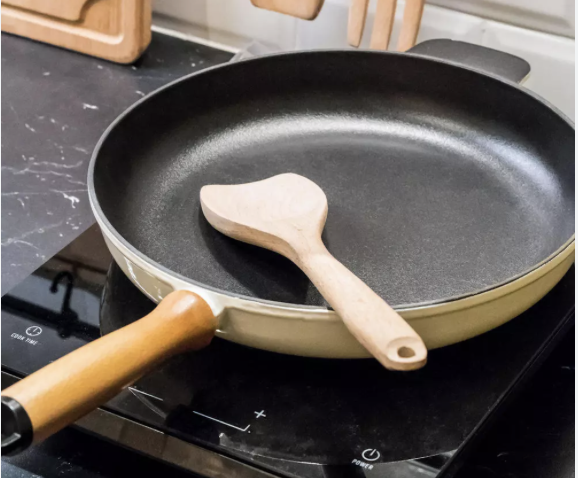
\includegraphics[width=.6\linewidth]{poel.png}
	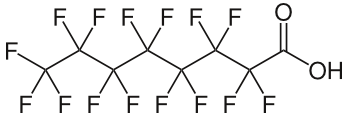
\includegraphics[width=.7\linewidth]{Perfluorooctanoic_acid.png}
	\captionof{figure}{Les PFAS à la base des revêtements des poêles en teflon}
\end{minipage}
}
\subsection{Des molécules identiques}

\begin{proposition}{Propriété 2 - molécules de synthése}
	Une molécule de synthèse reproduisant une molécule naturelle est exactement identique à cette dernière : même formule, mêmes propriétés physico-chimiques et mêmes dangers éventuels.
\end{proposition}

\subsection{Pourquoi synthétiser des espèces chimiques ? }

\begin{itemize}
	\item Fabriquer une molécule revient souvent moins cher que de l'extraire de son milieu naturel, mais aussi pour ne pas surexploiter les resources naturelles.
	\item L'industrie des parfums de luxe tient à utiliser les essences	naturelles et non leur équivalent de synthèse, même si elles sont plus coûteuses : le mélange naturel contient une plus grande variété de molécules, rendant le parfum final plus riche et complexe. 
\end{itemize}

\doc{1}{Les parfums - documentaire de C'est pas Sorcier}{
	\centering

\includegraphics[width=.2\linewidth]{LeparfumCestpasSorcier.png}
\captionof{figure}{\url{https://dgxy.link/fnzKP}}
}

\clearpage
\section{Comment synthétiser une espèce chimique au laboratoire ? }

\subsection{Le montage à reflux}

Une des techniques largement répandues pour synthétiser des molécules est le chauffage à reflux. 

\begin{definition}{Définition 7 - Le montage à reflux}
	Un montage à reflux permet de maintenir un mélange réactionnel à ébullition, en évitant les pertes de matière grâce au refroidissement des vapeurs, qui se liquéfient et retombent dans le ballon.
\end{definition}

\methode{3}{Étape de synthèse d'une molécule à l'aide du montage à reflux}{

\begin{enumerate}
	\item \textbf{Montage à reflux}: On porte à ébullition le milieu réactionnel jusqu'à la fin de la transformation chimique;\medskip
	
	\item \textbf{Extraction :} il faut séparer le produit désiré du milieu réactionnel. L'extraction peut être réalisée de deux façons en utilisant les \textbf{différences de solubilité} des espèces chimiques:
	\begin{itemize}
		\item Relargage : séparation en introduisant une autre espèce plus soluble avec le milieu réactionnel que l'espèce désirée.\medskip
		\item Extraction liquide/liquide : séparation de deux phases non miscibles.
	\end{itemize}
\end{enumerate}

L'extraction se fait généralement dans une verrerie très particulière que l'on appelle \textbf{l'ampoule à décanter}.
}
\vfill

\doc{2}{Schéma du montage à reflux}{

\begin{pspicture}[shift=2]
\psset{unit=.7cm} 
% \psgrid
\rput[t1](11,10){\large Réfrigérant à boule}
\psline[linewidth=.05]{->}(6.5,10)(3.2,10)
\psline[linestyle=dashed](7,9.3)(15,9.3)

\rput[t1](11,7){\large Ballon}
\psline[linewidth=0.05]{->}(6.5,7)(5,7)(3.5,5)
\psline[linestyle=dashed](7,6.3)(15,6.3)

\rput[t1](11,3){\large Chauffe ballon}
\psline[linestyle=dashed](7,2.3)(15,2.3)
\psline[linewidth=.05]{->}(6.5,3)(3,3)

\rput[t1](11,1){\large Support élévateur}
\psline[linewidth=.05]{->}(6.5,1)(3.2,1)
\psline[linestyle=dashed](7,0.3)(15,0.3)

\pstBallon[linewidth = .05, refrigerantBoulles,glassType=ballon,%
substance=\pstClouFer]
\psframe[fillstyle=solid,fillcolor=gray](-4.2,2)(0.2,1.8)
\psline(-4.2,1.8)(0.2,0)
\psline(0.2,1.8)(-4.2,0)
\psframe[fillstyle=solid,fillcolor=gray](-4.2,0)(0.2,-0.2)


\end{pspicture}

}	

\doc{3}{Schéma de l'ampoule à décanter}{
	\centering

	\psset{unit=.13cm} 
	\begin{pspicture}(-2,-6)(6,16)%\psgrid%
		\pstSupport
		\pstSeparateFunnel[OpenTap=false,bouchon]
	\end{pspicture}
	\hspace{2cm}
	\begin{pspicture}(-2,-6)(6,16)%\psgrid%
	\pstSupport \pstSeparateFunnel[OpenTap=false,bouchon=false,niveauLiquide1=-1,niveauLiquide2=10] \rput(0,-3){\pstTubeEssais[glassType=becher,aspectLiquide1=AqueoPhase]}
	\end{pspicture}
	\hspace{2cm}
	\begin{pspicture}(-2,-6)(6,16)%\psgrid% 
	\pstSupport \pstSeparateFunnel[OpenTap,bouchon=false,niveauLiquide1=1,niveauLiquide2=1] 
	\rput(0,-3){\pstTubeEssais[glassType=becher,aspectLiquide1=OrganicPhase,niveauLiquide1=30]} \pstSupport
	\end{pspicture}

}

\clearpage
\subsection{Analyse du produit obtenu}

	Une fois l'espèce synthétisée, isolée et purifiée, il est nécessaire de l'identifier pour vérifier qu'elle correspond bien à la molécule souhaitée. Différentes méthodes sont alors possibles:

	\begin{itemize}
		\item La chromatographie sur couche mince (CCM);
		\item La détermination de la température de changement d'état;
		\item La masse volumique;
		\item L'indice de réfraction; 
		\item Et bien d'autres ...
	\end{itemize}\medskip

	\doc{4}{Lecture d'un chromatogramme}{
	\begin{minipage}{.6\linewidth}
		$\bullet$ \textbf{Lecture verticale:} lorsqu'un dépôt se sépare en plusieurs tâches, l'échantillon testé est un mélange.\medskip

		$\bullet$ \textbf{Lecture horizontale:} sur une même plaque, une même espèce chimique présente dans des dépôts différents migre à la même hauteur.\medskip

		$\bullet$ Dans l'exemple ci-contre, M est un mélange des colorants E132 et E110 et d'un troisième colorant l' E122 qui sont des corps purs (une seule tâche par couleur). 
	\end{minipage}\hfill
	\begin{minipage}{.3\linewidth}
		\centering
		\includegraphics[width=1\textwidth]{CCM_TP.png}
	\end{minipage}
}
\vspace{3cm}

\section*{La synthèse d'une molécule en vidéo}

\doc{5}{Le montage à reflux - culture science}{

\centering

\includegraphics[width=.2\linewidth]{Reflux.png}
\captionof*{figure}{\url{https://dgxy.link/1XIA5}}
}


\doc{5}{L'extraction}{

\centering
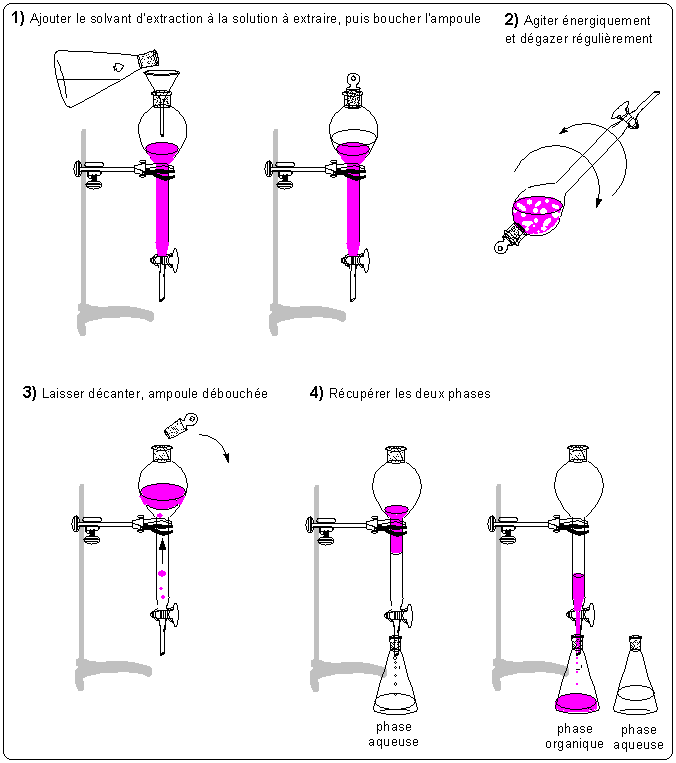
\includegraphics[width=.6\linewidth]{Extraction_liquide_liquide_Demirdjian_extraction.png}
\captionof*{figure}{\url{https://dgxy.link/uSJZ2}}
}
\end{document}